% Practice Test 23 — Virginia Edition
% Questions: 30 (15 MC + 15 SA)
% Generated by scripts/generate_practice_tests.py

\begin{practiceQuestion}{1-4-q05}{mc}
\begin{questionText}
If $y = 6x$, what is $y$ when $x = 7$?
\end{questionText}
\choiceA{$13$}
\choiceB{$36$}
\choiceC{$42$}
\choiceD{$48$}
\correctAnswer{C}
\explanation{$y = 6 \times 7 = 42$.}
\end{practiceQuestion}

\begin{practiceQuestion}{2-1-q30}{gsa}
\begin{questionText}
The circle graph shows how $200$ students get to school. How many students take the bus?

\begin{center}
\begin{tikzpicture}[scale=1.2]
  % Pie chart: Bus 45%, Walk 25%, Car 20%, Bike 10%
  \fill[funBlue!50] (0,0) -- (90:1) arc (90:252:1) -- cycle;
  \fill[funGreen!50] (0,0) -- (252:1) arc (252:342:1) -- cycle;
  \fill[funOrange!50] (0,0) -- (342:1) arc (342:414:1) -- cycle;
  \fill[funRed!50] (0,0) -- (54:1) arc (54:90:1) -- cycle;
  \draw[thick] (0,0) circle (1);
  \draw[thick] (0,0) -- (90:1);
  \draw[thick] (0,0) -- (252:1);
  \draw[thick] (0,0) -- (342:1);
  \draw[thick] (0,0) -- (54:1);
  % Labels
  \node[font=\small\bfseries] at (171:0.65) {Bus};
  \node[font=\small] at (171:0.4) {$45\%$};
  \node[font=\small\bfseries] at (297:0.65) {Walk};
  \node[font=\small] at (297:0.4) {$25\%$};
  \node[font=\small\bfseries] at (18:0.65) {Car};
  \node[font=\small] at (18:0.4) {$20\%$};
  \node[font=\small\bfseries] at (72:0.65) {Bike};
  \node[font=\small] at (72:0.4) {$10\%$};
\end{tikzpicture}
\end{center}
\end{questionText}
\correctAnswer{$90$ students}
\explanation{$45\%$ of $200$: $0.45 \times 200 = 90$ students take the bus.}
\end{practiceQuestion}

\begin{practiceQuestion}{2-2-q21}{sa}
\begin{questionText}
$91$ is $65\%$ of what number?
\end{questionText}
\correctAnswer{$140$}
\explanation{$\frac{91}{w} = \frac{65}{100}$. Cross-multiply: $65w = 9100$. Divide: $w = 140$.}
\end{practiceQuestion}

\begin{practiceQuestion}{2-3-q14}{mc}
\begin{questionText}
A gym membership increased from $\$45$ per month to $\$54$ per month. What is the percent increase?


\numberLine[1]{45}{55}
\end{questionText}
\choiceA{$9\%$}
\choiceB{$15\%$}
\choiceC{$18\%$}
\choiceD{$20\%$}
\correctAnswer{D}
\explanation{Change: $54 - 45 = 9$. Percent increase: $9 \div 45 = 0.20 = 20\%$.}
\end{practiceQuestion}

\begin{practiceQuestion}{2-7-q22}{sa}
\begin{questionText}
A lab experiment expected to produce $250$ mL but produced $240$ mL. Find the percent error.
\end{questionText}
\correctAnswer{$\approx 4.2\%$}
\explanation{$\frac{|250 - 240|}{240} \times 100 = \frac{10}{240} \times 100 \approx 4.17 \approx 4.2\%$.}
\end{practiceQuestion}

\begin{practiceQuestion}{3-2-q28}{gmc}
\begin{questionText}
Look at the table of deposits and withdrawals from a bank account.

\begin{center}
\begin{tabular}{|c|c|}
\hline
\textbf{Day} & \textbf{Transaction} \\
\hline
Monday & $+\$30$ \\
\hline
Tuesday & $-\$45$ \\
\hline
Wednesday & $+\$20$ \\
\hline
Thursday & $-\$15$ \\
\hline
\end{tabular}
\end{center}

If the account started at $\$0$, what is the balance after Thursday?
\end{questionText}
\choiceA{$\$110$}
\choiceB{$-\$10$}
\choiceC{$\$10$}
\choiceD{$-\$50$}
\correctAnswer{B}
\explanation{$0 + 30 + (-45) + 20 + (-15) = 30 + 20 - 45 - 15 = 50 - 60 = -10$. The balance is $-\$10$.}
\end{practiceQuestion}

\begin{practiceQuestion}{3-3-q15}{mc}
\begin{questionText}
Which subtraction problem gives a positive result?
\end{questionText}
\choiceA{$(-6) - 2$}
\choiceB{$3 - 11$}
\choiceC{$(-1) - (-9)$}
\choiceD{$(-5) - 3$}
\correctAnswer{C}
\explanation{$(-1) - (-9) = (-1) + 9 = 8$, which is positive.}
\end{practiceQuestion}

\begin{practiceQuestion}{3-4-q13}{mc}
\begin{questionText}
The temperature is $-6.4°$C. It rises $9.2°$C. What is the new temperature?
\end{questionText}
\choiceA{$-15.6°$C}
\choiceB{$15.6°$C}
\choiceC{$-2.8°$C}
\choiceD{$2.8°$C}
\correctAnswer{D}
\explanation{$-6.4 + 9.2 = 2.8°$C. Different signs: $9.2 - 6.4 = 2.8$, positive.}
\end{practiceQuestion}

\begin{practiceQuestion}{4-3-q08}{mc}
\begin{questionText}
Expand and simplify $2(x + 3) + 5$.
\end{questionText}
\choiceA{$2x + 8$}
\choiceB{$2x + 11$}
\choiceC{$2x + 10$}
\choiceD{$7x + 3$}
\correctAnswer{B}
\explanation{Expand: $2x + 6$. Add $5$: $2x + 6 + 5 = 2x + 11$.}
\end{practiceQuestion}

\begin{practiceQuestion}{4-4-q25}{sa}
\begin{questionText}
Show that $4(5x + 3)$ and $20x + 12$ are equivalent by expanding.
\end{questionText}
\correctAnswer{$4(5x + 3) = 4 \times 5x + 4 \times 3 = 20x + 12$}
\explanation{Distribute $4$: $4 \times 5x = 20x$ and $4 \times 3 = 12$. So $4(5x + 3) = 20x + 12$ \checkmark. They are equivalent.}
\end{practiceQuestion}

\begin{practiceQuestion}{5-4-q27}{gmc}
\begin{questionText}
Use the fraction bar model to solve: $\dfrac{2}{3}x = 8$. What is $x$?

\begin{center}
\begin{tikzpicture}[scale=0.6]
  % Full bar = x
  \draw[thick,fill=funBlue!15] (0,2) rectangle (12,3);
  \node at (6,2.5) {$x$};
  % 2/3 of bar highlighted
  \draw[thick,fill=funOrange!30] (0,0) rectangle (8,1);
  \node at (4,0.5) {$\frac{2}{3}x = 8$};
  \draw[thick,fill=gray!15] (8,0) rectangle (12,1);
  \node at (10,0.5) {$?$};
  % Dividers
  \draw[dashed] (4,0) -- (4,1);
  \draw[dashed] (4,2) -- (4,3);
  \draw[dashed] (8,0) -- (8,3);
  \node[below] at (2,-0.2) {$\frac{1}{3}$};
  \node[below] at (6,-0.2) {$\frac{1}{3}$};
  \node[below] at (10,-0.2) {$\frac{1}{3}$};
\end{tikzpicture}
\end{center}
\end{questionText}
\choiceA{$x = 12$}
\choiceB{$x = 16$}
\choiceC{$x = 10$}
\choiceD{$x = 5\dfrac{1}{3}$}
\correctAnswer{A}
\explanation{If $\frac{2}{3}x = 8$, then each $\frac{1}{3}$ of $x$ is $4$. So $x = 3 \times 4 = 12$.}
\end{practiceQuestion}

\begin{practiceQuestion}{5-5-q10}{mc}
\begin{questionText}
Solve $3x + 7 \leq 25$.
\end{questionText}
\choiceA{$x \leq \dfrac{32}{3}$}
\choiceB{$x \leq 6$}
\choiceC{$x \geq 6$}
\choiceD{$x \leq 9$}
\correctAnswer{B}
\explanation{Subtract $7$: $3x \leq 18$. Divide by $3$: $x \leq 6$.}
\end{practiceQuestion}

\begin{practiceQuestion}{5-6-q24}{sa}
\begin{questionText}
What inequality is shown by a closed circle at $-6$ with shading to the right?
\end{questionText}
\correctAnswer{$x \geq -6$}
\explanation{Closed circle means $-6$ is included, shading right means values greater than or equal to $-6$: $x \geq -6$.}
\end{practiceQuestion}

\begin{practiceQuestion}{6-1-q30}{gsa}
\begin{questionText}
A scale drawing of a soccer field is shown on the grid below. Each grid square represents $10$ m $\times$ $10$ m in real life. What is the actual perimeter of the field?

\begin{center}
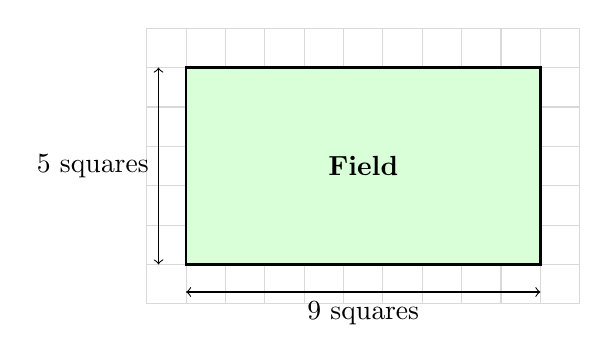
\begin{tikzpicture}[scale=0.5]
  \draw[step=1,gray!30,thin] (0,0) grid (11,7);
  \draw[thick,fill=green!15] (1,1) rectangle (10,6);
  \node at (5.5,3.5) {\textbf{Field}};
  \draw[<->] (1,0.3) -- (10,0.3);
  \node[below] at (5.5,0.3) {$9$ squares};
  \draw[<->] (0.3,1) -- (0.3,6);
  \node[left] at (0.3,3.5) {$5$ squares};
\end{tikzpicture}
\end{center}
\end{questionText}
\correctAnswer{$280$ m}
\explanation{Each square is $10$ m. Length: $9 \times 10 = 90$ m. Width: $5 \times 10 = 50$ m. Perimeter: $2(90 + 50) = 2(140) = 280$ m.}
\end{practiceQuestion}

\begin{practiceQuestion}{6-2-q22}{sa}
\begin{questionText}
A floor plan uses $1$ cm $= 6$ ft. On this plan, a room is $9$ cm long. On a second plan, the same room is $3$ cm long. What scale does the second plan use?
\end{questionText}
\correctAnswer{$1$ cm $= 18$ ft}
\explanation{Actual length: $9 \times 6 = 54$ ft. New scale: $54 \div 3 = 18$ ft per cm.}
\end{practiceQuestion}

\begin{practiceQuestion}{6-5-q25}{sa}
\begin{questionText}
A square pyramid has a base edge of $8$ cm. It is sliced parallel to the base halfway up. Is the cross-section larger, smaller, or the same size as the base?
\end{questionText}
\correctAnswer{Smaller than the base}
\explanation{A horizontal cut parallel to the base of a pyramid produces a similar shape that is smaller than the base. Halfway up, the cross-section is a $4$ cm square (half the edge length).}
\end{practiceQuestion}

\begin{practiceQuestion}{6-6-q21}{sa}
\begin{questionText}
Two vertical angles are $(7x + 1)°$ and $(5x + 13)°$. Find $x$ and the angle measure.
\end{questionText}
\correctAnswer{$x = 6$; the angles are $43°$}
\explanation{Vertical angles are equal: $7x + 1 = 5x + 13$. Subtract $5x$: $2x + 1 = 13$. Subtract $1$: $2x = 12$. Divide: $x = 6$. Angle: $7(6) + 1 = 43°$.}
\end{practiceQuestion}

\begin{practiceQuestion}{6-7-q11}{mc}
\begin{questionText}
Which of the following is true about all three rigid transformations (translation, reflection, rotation)?
\end{questionText}
\choiceA{They all change the size of the figure}
\choiceB{They all preserve the size and shape of the figure}
\choiceC{They all keep the figure's orientation the same}
\choiceD{They all move the figure to the right}
\correctAnswer{B}
\explanation{Translations, reflections, and rotations are all rigid motions — they preserve size and shape. Reflections reverse orientation, and rotations change direction, but all keep the figure congruent.}
\end{practiceQuestion}

\begin{practiceQuestion}{6-8-q22}{sa}
\begin{questionText}
Rectangle $PQRS$ is similar to Rectangle $WXYZ$. $PQ = 5$, $QR = 8$, $WX = 12.5$. Find $XY$.
\end{questionText}
\correctAnswer{$20$}
\explanation{Scale factor: $\frac{12.5}{5} = 2.5$. $XY = 8 \times 2.5 = 20$.}
\end{practiceQuestion}

\begin{practiceQuestion}{7-4-q28}{gmc}
\begin{questionText}
The diagram shows a figure made of a rectangle and a triangle. What is the total area?

\begin{center}
\begin{tikzpicture}[scale=0.5]
  \fill[funBlue!20] (0,0) -- (10,0) -- (10,4) -- (5,7) -- (0,4) -- cycle;
  \draw[thick,funBlue] (0,0) -- (10,0) -- (10,4) -- (5,7) -- (0,4) -- cycle;
  \draw[dashed,gray] (0,4) -- (10,4);
  \draw[thick,funRed,<->] (0,-0.7) -- (10,-0.7);
  \node[below,funRed] at (5,-0.7) {$10$ m};
  \draw[thick,funRed,<->] (10.7,0) -- (10.7,4);
  \node[right,funRed] at (10.7,2) {$4$ m};
  \draw[thick,funRed,<->] (5,4) -- (5,7);
  \node[right,funRed] at (5,5.5) {$3$ m};
\end{tikzpicture}
\end{center}
\end{questionText}
\choiceA{$40$ m$^2$}
\choiceB{$55$ m$^2$}
\choiceC{$70$ m$^2$}
\choiceD{$85$ m$^2$}
\correctAnswer{B}
\explanation{Rectangle: $10 \times 4 = 40$ m$^2$. Triangle: $\frac{1}{2} \times 10 \times 3 = 15$ m$^2$. Total: $40 + 15 = 55$ m$^2$.}
\end{practiceQuestion}

\begin{practiceQuestion}{7-5-q23}{sa}
\begin{questionText}
A shipping box is $12$ in by $8$ in by $6$ in. What is the total surface area?
\end{questionText}
\correctAnswer{$432$ in$^2$}
\explanation{$SA = 2(12 \times 8) + 2(12 \times 6) + 2(8 \times 6) = 192 + 144 + 96 = 432$ in$^2$.}
\end{practiceQuestion}

\begin{practiceQuestion}{7-6-q02}{mc}
\begin{questionText}
Which formula is used to find the volume of any prism?
\end{questionText}
\choiceA{$V = lwh$ only}
\choiceB{$V = Bh$}
\choiceC{$V = 2(lw + lh + wh)$}
\choiceD{$V = \frac{1}{3}Bh$}
\correctAnswer{B}
\explanation{The general formula for the volume of any prism is $V = Bh$, where $B$ is the area of the base and $h$ is the height.}
\end{practiceQuestion}

\begin{practiceQuestion}{7-7-q03}{mc}
\begin{questionText}
A cylinder has a diameter of $8$ cm and a height of $5$ cm. What is its volume? Use $\pi \approx 3.14$.
\end{questionText}
\choiceA{$100.48$ cm$^3$}
\choiceB{$200.96$ cm$^3$}
\choiceC{$251.2$ cm$^3$}
\choiceD{$401.92$ cm$^3$}
\correctAnswer{C}
\explanation{$r = 4$ cm. $V = \pi r^2 h = 3.14 \times 16 \times 5 = 251.2$ cm$^3$.}
\end{practiceQuestion}

\begin{practiceQuestion}{8-1-q21}{sa}
\begin{questionText}
A random sample of $50$ apples from an orchard found that $6$ were bruised. If the orchard has $3{,}000$ apples, about how many are bruised?
\end{questionText}
\correctAnswer{$360$}
\explanation{$\frac{6}{50} = 12\%$. Then $12\%$ of $3{,}000 = 360$.}
\end{practiceQuestion}

\begin{practiceQuestion}{8-3-q22}{sa}
\begin{questionText}
Team A: mean $60$, MAD $4$. Team B: mean $70$, MAD $3$. Is the difference in means meaningful? Explain briefly.
\end{questionText}
\correctAnswer{Yes; the means are about $2.5$ to $3.3$ MADs apart}
\explanation{Difference $= 10$. Using MAD of $4$: $\frac{10}{4} = 2.5$. Using MAD of $3$: $\frac{10}{3} \approx 3.3$. Both are greater than $2$, so the difference is meaningful.}
\end{practiceQuestion}

\begin{practiceQuestion}{8-4-q05}{mc}
\begin{questionText}
Data set: $20, 22, 25, 27, 30, 32, 35$. What is the IQR?
\end{questionText}
\choiceA{$15$}
\choiceB{$10$}
\choiceC{$7$}
\choiceD{$5$}
\correctAnswer{B}
\explanation{$Q_1 = 22$, $Q_3 = 32$. IQR $= 32 - 22 = 10$.}
\end{practiceQuestion}

\begin{practiceQuestion}{8-5-q22}{sa}
\begin{questionText}
How many data values are shown in this stem-and-leaf plot?

Stem $5$: $1\;\;3\;\;5$ \quad Stem $6$: $0\;\;2\;\;4\;\;7\;\;8$ \quad Stem $7$: $1\;\;6$ \quad Stem $8$: $0$
\end{questionText}
\correctAnswer{$11$}
\explanation{Count leaves: $3 + 5 + 2 + 1 = 11$.}
\end{practiceQuestion}

\begin{practiceQuestion}{9-3-q11}{mc}
\begin{questionText}
Tyler draws a card from a standard deck, records the suit, and replaces it. He does this $52$ times. Hearts appear $16$ times. What is the experimental probability of drawing a heart?
\end{questionText}
\choiceA{$\frac{13}{52}$}
\choiceB{$\frac{16}{52}$}
\choiceC{$\frac{16}{36}$}
\choiceD{$\frac{4}{13}$}
\correctAnswer{B}
\explanation{$P = \frac{16}{52} = \frac{4}{13} \approx 0.308$. Note: $\frac{16}{52}$ and $\frac{4}{13}$ are equivalent, but B directly shows the experimental data.}
\end{practiceQuestion}

\begin{practiceQuestion}{9-6-q20}{sa}
\begin{questionText}
A coin is flipped and a die is rolled. What is the probability of getting tails and a $1$? Write your answer as a fraction.
\end{questionText}
\correctAnswer{$\frac{1}{12}$}
\explanation{$P(\text{tails}) = \frac{1}{2}$, $P(1) = \frac{1}{6}$. $P = \frac{1}{2} \times \frac{1}{6} = \frac{1}{12}$.}
\end{practiceQuestion}

\begin{practiceQuestion}{9-7-q12}{mc}
\begin{questionText}
How does increasing the number of trials in a simulation affect the results?
\end{questionText}
\choiceA{The results become less reliable}
\choiceB{The experimental probability gets closer to the theoretical probability}
\choiceC{The results stay exactly the same}
\choiceD{The simulation takes less time}
\correctAnswer{B}
\explanation{More trials produce more reliable estimates. The experimental probability approaches the theoretical value as trials increase.}
\end{practiceQuestion}
